\chapter{JPDI Architecture}
Jaqpot Protocol of Data Interchange, shortly JPDI, 
is a brand new feature of JAQPOT that allows developers 
of QSAR-related or machine learning algorithms to 
integrate their implementations in JAQPOT so that these
can be used by JAQPOT for QSAR.


n Jaqpot3 a Dataset is frequently consumed in ARFF format by the Dataset service, 
as Weka is the main QSAR engine and Weka Instances can easily be created by ARFF. 
Then all pre-processing is done on those Instances and the Algorithm training as well. 
ARFF and Instances are quite convenient when applying Weka algorithms on a Dataset, 
but not a generic solution to accommodate different Algorithmic engines.
 
Jaqpot Quattro introduces OpenCPU, an HTTP proxy to R, a language that has 
interesting packages regarding QSAR. In order to interact with R, Jaqpot must consume an 
OpenCPU resource that masks an R function and provide a Dataset in Json format as input 
to that function. The input Dataset could also be enriched by some extra detail, as to 
which of the Features is to be predicted, and various parameters if 
needed by the specific algorithm.


\section{JPDI Specification}
Algorithm implementation could be decoupled from Jaqpot. 
Taking example from the OpenCPU solution, we could create different 
individual services for each QSAR engine and it’s algorithms. Then a user could 
use Jaqpot's Algorithm service to create/update/remove Algorithm resources at will. 

\begin{figure}[h]
 \centering
 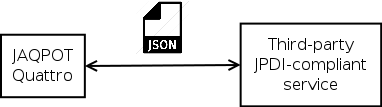
\includegraphics[keepaspectratio=true,width=0.6\textwidth]{figures/JPDI_general.png}
\end{figure}

As shown in the above figure, JAQPOT communicates with 
third-party, external, and independent WSs over HTTP
using a very simple REST interface that we will discuss
hereafter and uses JSON as the standard data exchange format.
The essential principles of JPDI are the following:


\begin{enumerate}
 \item The JPDI API is super-easy for non-expert programmers to 
 implement (so that people can get to integrate their algorithms in
 JAQPOT); JPDI compliant services do not need to maintain a database
 or implement a queue of asynchronous jobs\footnote{this would be
 required for someone to implement an OpenTox-compliant WS, but building
 a JPDI-compliant WS is piece of cake!},
 \item JAQPOT and JPDI services are developed independently,
 \item Services communicate over HTTP exchanging JSON files
 \item Services exchange only what is necessary in the way the JPDI
 specs mandate,
 \item Integration is seamless: JPDI services are plug-in, plug-out 
 and can be added or removed from JAQPOT Quattro at any time,
 \item Third-party services are absolutely free to decide how they
 want to store their models on JAQPOT (the can store them even in 
 custom binary formats).
\end{enumerate}


\section{Training with JPDI-compliant WSs}
Training with a JPDI-compliant WS is explained in this section.
As we see in the following picture, the JAQPOT User Interface 
in collaboration with the JAQPOT Web Services prepares all necessary
data to be sent to the JPDI training service. The following input is
provided to the training service:

\begin{enumerate}
 \item The training dataset where the target feature is 
 indicated to the training service, 
 \item tuning parameters of the algorithm as requested by JPDI
 \item other metadata that \textit{may} be useful to the JPDI service
 (\textit{e.g.}, the URI of the training dataset).
\end{enumerate}
\begin{figure}
\centering
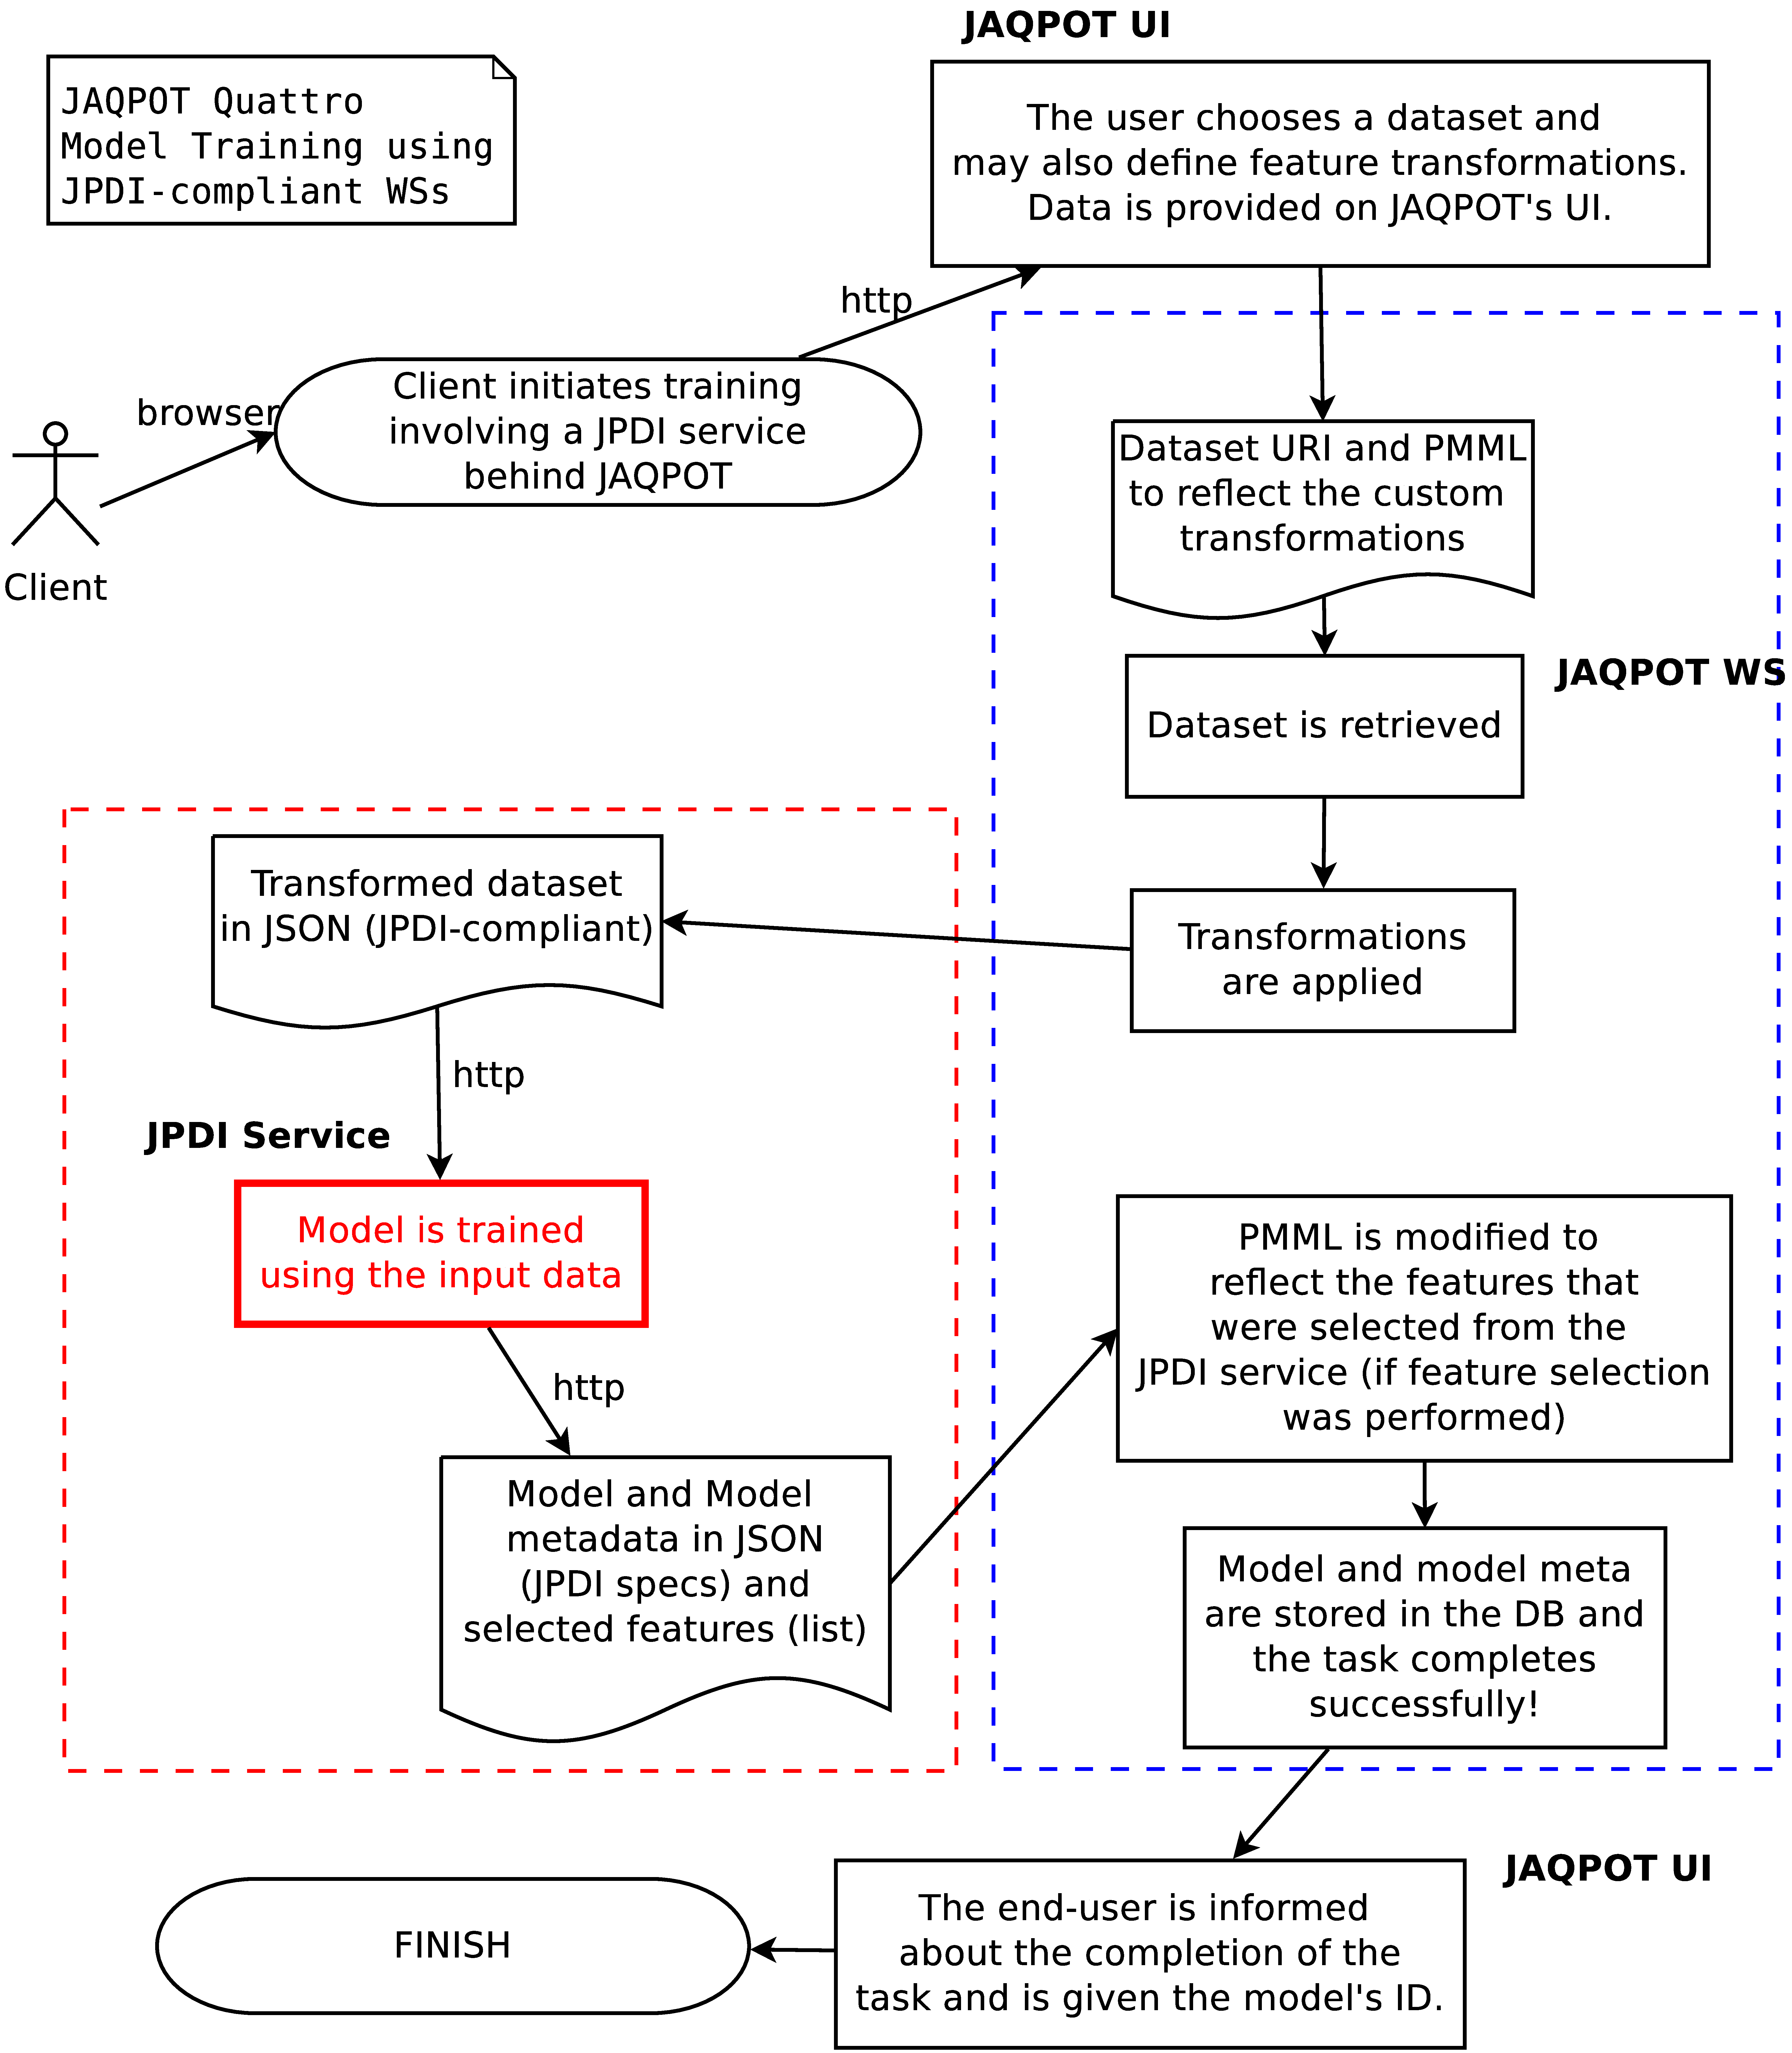
\includegraphics[keepaspectratio=true,width=0.999\textwidth]{figures/JPDI_training.eps}
\end{figure}
Here is an example of a training request in JSON. 
A training service has all that it needs to train a
new machine-learning model. Notice that missing values are set
to \texttt{null}.
Algorithm-specific parameters are passed to the training service
in the same JSON documents.

\begin{lstlisting}[language=json]
 {
    "jpdi_verion" : "1.0.0",
    "data" : {
      "/compound/1/conformer/11": 
	  [1.23, 2.44, 5.01, null, 0.07, 0.94],
      "/compound/2/conformer/31": 
	  [9.31, 1.90, 8.11, 0.05, 0.21, 0.88],
      "/compound/3/conformer/90": 
	  [8.10, 0.67, 7.10, 0.00, 0.44, 0.67],
      "/compound/4/conformer/45": 
	  [3.91, 1.03, 8.37, 0.28, null, 0.99]
    },
    "parameters" : {
      "lambda" : 1,
      "c" : 0.8,
      "epsilon" : 0.1,
      "tolerance" : 0.00001
    }
}
\end{lstlisting}

The, the JPDI service will process this information and will
produce a model that can be stored in any format (this is to 
be decided by the JPDI service developers). We suggest PMML 
if it is possible that the model can be serialized in this 
format. If the model is to be serialized in some custom binary
format we recommend that it is encoded in \texttt{Base91} (although,
it is completely up to the service provider to decide that).


Once the model is trained, the JPDI service will return it
to JAQPOT in JSON in which the actual model is encoded.
Here is an example:

\begin{lstlisting}[language=json]
{
  "feature_selection": true,
  "selected_features" : [1, 2, 5],
  "model":"FSKHEKJFBADNFBDABDABSD..."
} 
\end{lstlisting}

The actual model data is stored under \texttt{model}; of course
JAQPOT cannot interpret this data, so the JPDI service is also 
responsible to provide predictions when a user needs to use 
the model. Notice that here the JPDI service also performed 
feature selection and selected the first, the 
second and the fifth features among the ones that were given to it%
\footnote{The JPDI service doesn't (need to) know what the input features
really are, so their URIs are useless to it. Likewise, it can perform
feature selection without having access to the feature definitions/metadata.
The take-away message is that JPDI training services do \textbf{only} training.}.
Now this model is stored in the DB of JAQPOT and a new model resource is created
and is assigned a new URI.

In this example of model training, since the training
WS has selected these 3 features as input features, 
when one needs to do a prediction, these exact features 
in this very order need to be sent to the JPDI service.
This is done in a very easy way as we see in the training 
workflow: the PMML file is modified to store the necessary
feature transformations and feature selection so as to
create a dataset for prediction.





\section{Prediction with JPDI-compliant WSs}


\section{Registration of new algorithms}
New algorithms need to be \textit{registered} on JAQPOT Quattro
so that JAQPOT knows how to invoke them. This is specified in 
a very simple manner on registration. JPDI algorithms
are registered by a POST method applied on \texttt{/algorithm}.

\begin{lstlisting}[language=json]
{
  "title": "SuperTraining",
  "description" : "this is a mighty algorithm",
  "author" : "W.Y. Chung",
  "parameters": [
    {
      "name" : "x",
      "description" : "this is x",
      "default_value" : 0.045,
      "type" : "numeric",
      "scope" : "optional"
    },
    {
      "name" : "y",
      "description" : "this is y",
      "default_value" : true,
      "type" : "boolean",
      "scope" : "optional"
    },
  ]
} 
\end{lstlisting}

